
\chapter{基于多模态深度学习的三维形状识别与检索}

在本文中,我们提供了一个综合考虑三维形状的外在属性和内在特征的解决方案。 我们提出了一个新的方案来融合3D形状的不同形态数据到深度学习框架。 其核心思想是运用深度学习技术,融合三维模型的几何特征和视觉特征,并进行提取得到具有强表达能力的高层特征。简而言之,卷积深度置信网络(CDBN)和卷积神经网络(CNN)分别用于从基于几何的模态和基于视图的模态学习三维形状。 接下来,这两种模式利用受限玻尔兹曼机(RBM)融合以获得具有更强判别力特征。其中包括以下三个主要部分:
\begin{enumerate}
\item 基于视觉的特征学习
\item 基于几何的特征学习
\item 多模态融合
\end{enumerate}


这个框架有三个好处,如下所述。 首先,融合不同的模式,可以全面理解3D形状。 第二,在不同的特征提取程序中使用不同的深度学习技术,充分利用各种深度学习方法从三维模型中提取不同特征的属性。 第三,与其他需要手动调整参数以获得最佳性能的机器学习方法不同,在整个学习过程中没有要调整的参数。 提出的方案是自动学习的。

尽管上述方法在分类,匹配和检索方面取得了巨大的进步,但是在更多领域应用3D对象还远远不能令人满意。主要问题在于基于几何的方法和基于视图的方法仅使用3D对象的部分信息。 详细而言,基于几何的方法利用了3D模型本身的复杂拓扑结构和几何特性,而忽略了三维物体之间的视觉相似性。 相反,基于视图的方法仅考虑来自不同观看图像的模型的视觉特性。 为了克服各自缺点,我们尝试使用深度学习技术来学习和融合几何和视图方面的不同模式。 这项工作的主要贡献可以归结为两个方面:
\begin{itemize}

\item 多模态融合:为了进一步提高性能,采用多模态融合学习三维形状内在的非线性关系。 通过融合多模描述符,可以封装互补的视觉和几何信息,提高分类和检索的准确性。
\item 深度特征:CNN和CDBN用于提取3D形状的视觉和几何特征。 CNN具有较强的视觉特征提取能力,而CDBN具有从3D对象中产生高性能特征的能力。我们的框架充分利用了CNN和CDBN,因此可以提取更全面的描述。

\end{itemize}



\begin{figure*}[htbp]
\begin{center}
 \includegraphics[width=0.98\linewidth]{figures/cnn-cdbn-dbn-crf-new14}
 \end{center} \vspace{-4mm}
\caption{基于多模态深度学习的三维形状识别与检索的流程图(展示了离线的训练过程)% The multi-modal feature data association part is detailly shown in Fig. \ref{fig_multi-modal_structure})
} 
\label{flowchart}
\end{figure*}

几何和视觉信息是三维形状研究的两个重要方面。在我们的框架中,我们分别提取这两个类型的描述符,然后将它们融合生成具有高判别性和有效性的3D MMF。该方法的流程图如图\ref{flowchart}所示,表明提出的多模态特征融合体系结构包含两个模态输入:几何描述符和视觉描述符。传统的几何特征是使用复杂的三维形状结构应对大量丰富点设计的。在预处理中下采样是减少产生各种特征的计算时间的有效方法。在我们的框架下,CNN和CDBN模型的预处理是没有下采样方法产生的体素化和深度图像。在几何特征提取中,三维形状从网格形式转换成接近原始三维对象的体素表示,因此我们不需要下采样。在视觉特征提取中,我们以深度图像作为输入,由于将三维形状转换为多幅图像,也不需要下采样。接下来分步介绍。


\section{所涉及的深度学习方法介绍}

\subsection{卷积神经网络(CNN)}

卷积神经网络(CNN)是一种有效的模式识别领域的方法。传统模式识别的方法中,图像的预处理是一件非常复杂的事情,例如,平滑,锐化等操作,因此增加了图像处理的复杂性,效率不高。CNN可以直接对图像进行处理,其区域连接和权值共享更是提高了CNN的图像处理的能力,加了整个模型的计算性能。CNN如此优秀的表现,得益于Hubel和Wiesel的贡献。他们发现在猫脑皮层中用于局部敏感和方向选择的神经元有这种区域连接的网络,不仅有效地降低反馈神经网络的复杂性而且增加了预测的精度。

% 卷积神经网络是近年发展起来,并引起广泛重视的一种高效识别方法。20世纪60年代,Hubel和Wiesel在研究猫脑皮层中用于局部敏感和方向选择的神经元时发现其独特的网络结构可以有效地降低反馈神经网络的复杂性,继而提出了卷积神经网络(Convolutional Neural Networks-简称CNN)。现在,CNN已经成为众多科学领域的研究热点之一,特别是在模式分类领域,由于该网络避免了对图像的复杂前期预处理,可以直接输入原始图像,因而得到了更为广泛的应用。 K.Fukushima在1980年提出的新识别机是卷积神经网络的第一个实现网络。随后,更多的科研工作者对该网络进行了改进。其中,具有代表性的研究成果是Alexander和Taylor提出的“改进认知机”,该方法综合了各种改进方法的优点并避免了耗时的误差反向传播。

CNN神经网络作为第一个被成功训练并且应用的多层神经网路结构,具有较强的容错、自学习以及并行处理能力。最初是为识别二维图像而设计的多层感知器,模仿生物神经网络的局部链接和权值共享网络降低了神经网络的复杂度,减少权值数量,使网络对于输入具备一定的鲁棒性。CNN是一种多层的神经网络,具有很强的抽取图像特征能力,其网络结构具有很强的自学习和并行处理的能力。1962年Hubel和Wiesel通过对动物的视觉皮层细胞进行研究,提出了感知域的概念,用以能够使得神经元收到刺激而进行反馈的区域,同时这也说明一点,神经元的最初感知是发生在局部区域的。后续的相关研究相继提出简单单元(Simple Cell)和复杂单元(Complex cell)。简单单元只对方向的边缘产生响应,复杂的单元除了对方向的边缘产生响应,而且具有一定的空间不变的属性。基于感知域,神经认知机模型被提出,并且将其应用于计算机视觉中的视觉模式分类任务。神经认知机首先用多个模式来表示一个模式,接着以分层的方式对这些模式进行处理,通过不断的尝试将该视觉模型化,让其能够应对物体的偏移、扭曲等变形的识别。

基于认知机模型,世界的各地研究者提出了多种卷积网络形式用于视觉分类与识别。近年来,Yann LeCun教授提出的卷积神经网络是当前最为流行的一种形式,该网络成功应用于语音识别和图像分类等问题,推动了深度学习的发展。 CNN在神经网络的基础上,采用了局部感知野和权值共享的思想,有效地降低了传统前馈神经网络的复杂程度,并使用降采样层(又称作pooling层)来增加网络的平移不变性。

\textbf{CNN基本网络结构} 

卷积神经网络是一种多层的前馈网络,每一层由多个二维平面组成,每个平面再由多个神经元组成,如图\ref{cnn}。网络中卷积层(Convolutional Layer,C)和抽样层(Subsampling Layer,S)交替出现,相当于生物视觉系统中的简单单元和复杂单元交替出现。网络的最后一层为全连接方式的神经网络,输出层的维度对应数据中需要进行分类的类别数。

卷积层:该层为网络的特征提取层,每个卷积层包含多个神经元(C),每个神经元只对前一层的网络相应的局部位置进行特征提取,这体现在该神经元与前一层局部区域的连接权重上。相比较全连接的神经网络模型,这种局部连接的方式可以大大降低整个网络的参数。为了更加有效的训练整个网络,整个网络设计时采用权值共享的基本策略:即神经元对同一层所有区域的感知权值是相等的。特征映射结构采用Sigmoid函数作为卷积网络的激活函数,使其具有位移不变性的特点。

抽样层:该层为网络的特征映射层,每个卷积层包含多个神经元(S),网络的每个计算层由多个特征映射组成,每个特征映射为一个平面,平面上所有的神经元权值相等。
通过卷积层(C-层)和采样层中(S-层)交替进行特征提取,使得训练出来的特征对输入数据具有很高的畸变容忍能力。

\begin{figure*}[htbp]
\begin{center}
 \includegraphics[width=0.98\linewidth]{figures/cnn}
 \end{center} \vspace{-4mm}
\caption{卷积神经网络结构} 
\label{cnn}
\end{figure*}



\textbf{CNN训练学习} 

\begin{enumerate}
\item \textbf{卷积层。} 图像本质是一种由像素值排列起来的二维(或者多维)矩阵,是现实世界的一种数字化表现形式。由于图像的统计特性是有一定规律的,在图片中某一区域学习得到的局部特征同样能应用于另一区域。图\ref{conv}展示了图像卷积的过程。 

\begin{figure*}[htbp]
\begin{center}
 \includegraphics[width=0.5\linewidth]{figures/卷积过程}
 \end{center} \vspace{-4mm}
\caption{图像卷积过程} 
\label{conv}
\end{figure*}

在CNN网络中,原始输入图像(或者特征图)$x$ 经卷积核$W$ 处理之后,会生成新的特征图,此过程能够表示为
\begin{equation}
 I = f(x \otimes W)
\end{equation}
式中, 为$\otimes $为卷积操作, $I$为卷积单元处理后的结果, $f$为非线性变换函数。

\item \textbf{池化层降采样过程。} 该层对卷积层所产生的特征图进行下采样操作, $N$个输入特征图对应$N$个输出特征图,只是每个输出特征图的尺寸相比较原来变小,抽样层定义如下:

\begin{equation}
  a_j^l  =\sigma (\beta_j^l down(a_j^{l-1}) + b_j^l)
\end{equation}

公式中$down()$为下采样操作,对输入图中每个不重复的$n\times n$ 得图像块求和得到一个输出值,输出图的长和宽都是输出图的$1/n$ ,每个输出有一个乘性偏置$\beta$ 和偏置$b$ 。只要得到抽样层的灵敏度图,就可以求解出偏置参数$\beta$ 和偏置$b$的梯度。

卷积操作虽然能够有效降低整个网络的参数,但是对于图像处理来说,参数量仍然非常巨大。CNN有一个巧妙的安排,在卷积之后再进行池化操作。池化操作是对卷积出来的特征进行聚合的,从而进一步降低参数的个数。一般来说,最大池化、均值池化、随机池化是比较常见的。池化的作用不仅能降低维度而且能防止过拟合的作用,使特征具有平移鲁棒性。

% 通过卷积的方法得到输入图像的特征图之后,可以利用这些特征完成各种计算机视觉的任务。但如果直接使用这些特征图,会使得特征的维度非常高,训练一个高维度输入的模型十分不方便,而且容易出现过拟合。为了解决上面这个问题,可以对图像中某一区域的特定特征进行聚合操作,称之为池化(pooling),这种做法可以降低特征的维度,同时还能在一定程度上改善过拟合。常用的池化方法有最大值池化、均值池化和随机池化几种方法,其中最大值池化方法在卷积神经网络中应用较广。卷积操作之后进行降采样的做法,是CNN模型的显著特点。卷积层的功能为从原始图像中捕捉特征信息,减少无效信息的强度,而降采样层的功能是负责降维,减小计算量,同时保证了原始图像的平移鲁棒性。

\item \textbf{CNN的优势。} 在图像的识别处理过程中,传统的神经网络对图像的处理是使用全链接的。全链接得的最大的弊端就是需要学习的参数特别巨大,例如$1000 \times 1000$ 的图像,如果与$10^6$的隐藏层节点进行全链接,那么参数的数量将是成指数级别进行上涨的,那是将会有$10^{12}$个参数。面对如此巨量的参数,传统的神经网络难以进行有效的学习。CNN的卷积操作弥补这一弊端,CNN提出了区域连接和权值共享这两个技术。区域连接指神经网络的不是所有节点进行连接的,而是选择部分区域进行,这样有效的减少了参数,但同时CNN会在高层的时候对这些局部参数进行融合,进而弥补部分区域的信息的缺失,同时权值共享使得卷积核对不同的区域所有的参数可以共享,对于提取出来的参数不同部分是可以共享的。CNN使得对图像的处理效率更高,效果更好。

%由于传统的前馈神经网络全连接特性,当用于处理图像数据时,计算量是十分巨大的。比如一幅 $1000 \times 1000$ 的图像,将其转化为像素的一维向量后,将含有 $10^6$个元素,如果隐藏层节点数目也为 $10^6$,那么单层神经网络的参数数量就为 $10^12$个,这样巨大的参数个数会导致整个神经网络无法训练。为使神经网络算法对图像可用,必须减少网络中权值边的个数,CNN使用区域连接和权值共享思想来达到这一目的,这两种方法可以有效减少网络中的连接边数,区域连接和权值共享等价于CNN中的卷积层操作。换角度看,CNN中的卷积层操作实质上是区域连接和权值共享思想的具体实现。
%局部连接是指网络中的任意节点并不一定要与前一层的所有节点都有权值边相连,有可能只与部分节点相连接,只对图像的局部特性进行处理,在更高层中完成对图像区域信息的整合,就可得到图像的全局信息。在图像中某一部分学习得到的特征同样能应用于图像中其它部分,这就是连接边权值共享的基本原理。权值共享使得在CNN的每一个特征图(或者原始图像)内部,所有与卷积核大小相同的图像块所对应的连接边权值是完全一样的。对于CNN模型来说,区域连接和权值共享策略降低了网络训练的难度,使得训练一个有效的多层CNN网络具备了可能性。

\end{enumerate}

\subsection{深度置信网络(DBN)}
深度置信网络DBN是一种全连接网络,网络的训练过程就是优化其能量函数达到最小的过程。波尔兹曼机(BM)是一种非监督学习技术,常常被用作数据挖掘方面的处理。但是由于其隔层的节点之间的进行了层内的连接,使得BM的训练学习效率低,使得这种方法难以被广泛应用。Smolensky为了解决其效率低下的问题,将层内节点之间的连接全部去掉,提高了网络的学习效率,同时层间之间全链接,这种神经网络被称为限制性波尔兹曼机(RBM)。

RBM包含可使层、隐藏层,层内无连接,层间全链接。当隐藏层神经元足够多的时候,RBM可以拟合离多数散分布。RBM的提出是对BM的一个重大进步,然而,RBM还是没有得到广泛应用。究其原因,就是训练的时候仍然有诸多困难,进而难以高效的训练神经网络。Hinton针对这种问题,提出对比散度(CD)算法。有效的解决了RBM不能高效训练的问题,使得其在分类、回归、降噪、高维时间序列分析、图像特征提取、协同过滤等方面取得了优秀的表现。Hinton在对RBM研究的基础上,又提出了将多个RBM进行堆叠的想法,进而提出了深度信念网络(DBN),DBN的提出为神经网络参数的初始化提供了有力的工具。

% 这类网络首先起源于Holpfield网络,这是一种全联接的网络,神经元之间进行全连接,我们可以给这个网络定义一个能量函数,神经网络的学习任务就是使能量函数达到最小值。这类网络典型的成功应用是担货郎问题,即有N个地点,每个地点间都有道路相通,担货郎必须把货物送到每个地点,通过Holpfield网络,可以有效地找到最佳路径。但是即使是对于二值(神经元只能处在0或1状态),全联接网络的状态也2的N次方个状态,要从这些状态中找到找到能量函数的最小值,难度相当大,大家一定还记得国际象棋发明者,向国王讨赏的典故吧,一个64个方格的棋盘,连全世界总粮食产量都填不满,可见这个问题的复杂性。与此同时,根植于统计力学模型的波尔兹曼机(BM)也开始流行起来。在这种网络中,神经元的输出只有激活和未激活两种状态,用0或1来表示,各个神经元的输出值由概率纺计模型给出。

%由实践来看,波尔兹曼机(BM)具有强大的非监督学习能力,可以发现数据中潜在规则,理论上来讲,非常适合于数据挖掘领域应用。便是由于是全连接网络,导致这种网络的训练时间非常长,没有高效的学习算法,直接制约了这种网络的应用。后来Smolensky引入了限制性波尔兹曼机(RBM)模型,其主要思想就是去掉了波尔兹曼机中层内连接。限制性波尔兹曼机(RBM)具有一个可见层,一个隐藏层,层内神经元间无连接,层间神经元全连接。

%限制性波尔兹曼机(RBM)中,输入信号通过可见层输入到网络中,此时传播到隐藏层后,各隐藏层神经元的激活是互相独立的,同理在给定隐藏层信号后,反向传播到可见层时,可见层神经元的激活也具有独立性。可以从理论上证明,这种网络结构,只要隐藏层神经元节点足够多,限制性波尔兹曼机(RBM)可以拟合任意离散分布。虽然在理论上RBM很好,但是一直由于没有高效的学习算法,限制性波尔兹曼机(RBM)并没有得到广泛应用。但是深度学习之父Hinton在2002年提出了对比散度(CD)算法,使限制性波尔兹曼机(RBM)具备了快速学习的能力。从此,RBM得到了广泛的应用,出现了各种对比散度算法的变种,使得算法收敛性更高。与此同时,波尔兹曼机(RBM)在分类、回归、降噪、高维时间序列分析、图像特征提取、协同过滤等方面,得到了广泛的应用。另外,Hinton在2006年提出,将限制性波尔兹曼机(RBM)堆叠起来,形成深度信念网络(DBN),通过逐层训练RBM网络,将训练好的RBM网络堆叠成深度学习网络,可以得到非常好的初始参数值,有效地解决了大型神经网络训练速度慢的问题,是当前的研究热点之一。

\textbf{受限制的玻尔兹曼机RBM}

之所以说他是受限,是应为在RBM内取消了可见层和隐含层的层内连接,虽然BM具有强大的无监督学习能力,能过学习复杂的规则,但是因为层内连接,使得整个学习过程消耗漫长的时间。所以Smolensky发明了RBM是学习时间大大缩减。也为后面的DBN奠定了基础。

RBM有一个可见层和一个隐含层,通过上面的BM到RBM的转变使得RBM具有了一个很好的特性:在给定可见层单元状态时,各隐含单元的激活条件独立,反之,在给定隐含层单元的状态时,各隐含层激活条件也是独立的。虽然这样RBM所表示的分布仍是无法有效计算的,但是我们可以通过Gibbs采样使其得到服从RBM分布的随机样本。

RBM的可见层用v表示,用于接收输入信号,隐藏层由h表示,可以视为是输入信号的特征提取器。我们在前面讨论过,制约神经网络大规模应用的一个瓶颈之一,就是很难为研究问题找到合适的特征,而RBM则是通过无监督学习方式,自动找到研究问题的最佳特征,因此对于研究者们而言,具有非常大的吸引力,这也是为什么RBM在近些年来如此火的原因。我们设定可见层神经元为二值变量,即,隐藏层单元同样为二值变量,即,假定可见层有m个神经元,用下标i代表第j个神经元,隐藏层有n个神经元,用下标j表示第j个神经元。

我们可以定义网络的能量函数为
%
\begin{equation}
 E(v,h|\theta) = - \sum_{i=1}^n \sum_{j=1}^m v_jW_{ij}h_i - \sum_{j=1}^m b_j v_j - \sum_{i=1}^n c_i h_i,
\end{equation}
%
上式中为网络参数,均为实数,$W_{ij}$为可见层神经元i到隐藏层神经元j的连接权值,$b_j$为可见层第j个神经元的偏置,$c_i$为隐藏层第i个神经元的偏置。


\textbf{深度信念网络}
在机器学习的模型分类中,大抵可以分为两类,生成模型和判别模型。简单来说,生成模型刻画的是数据和标签的联合分布,而判别模型对于由数据预测类别进行了刻画。传统DBN进行训练的时候,弊端很多。例如,样本集标签必不可少,收敛慢,可能会收敛与局部最优等等问题。

DBNs由多个限制玻尔兹曼机(Restricted Boltzmann Machines)层组成。这些网络被“限制”为一个可视层和一个隐层,层间存在连接,但层内的单元间不存在连接。

% 隐层单元被训练去捕捉在可视层表现出来的高阶数据的相关性
% 首先,先不考虑最顶构成一个联想记忆(associative memory)的两层,一个DBN的连接是通过自顶向下的生成权值来指导确定的,RBMs就像一个建筑块一样,相比传统和深度分层的sigmoid信念网络,它能易于连接权值的学习。在最高两层,权值被连接到一起,这样更低层的输出将会提供一个参考的线索或者关联给顶层,这样顶层就会将其联系到它的记忆内容。而我们最关心的,最后想得到的就是判别性能,例如分类任务里面。
% 
% 在预训练后,DBN可以通过利用带标签数据用BP算法去对判别性能做调整。在这里,一个标签集将被附加到顶层(推广联想记忆),通过一个自下向上的,学习到的识别权值获得一个网络的分类面。这个性能会比单纯的BP算法训练的网络好。这可以很直观的解释,DBNs的BP算法只需要对权值参数空间进行一个局部的搜索,这相比前向神经网络来说,训练是要快的,而且收敛的时间也少。

卷积置信网络CDBN(Convolutional Deep Belief Networks)是DBN网络的拓展之一。DBN在图像训练的过程中,仅仅对原始数据进行向量化,即就是将二维化的图像信息转化为一维的向量信息。这种操作很明显的一个弊端就是丢失了二维图像信息的空间结构化信息。为了弥补这方面的不足,CDBN别来学习图像信息的结构化信息,卷积操作对于原始数据不仅仅是学习其直接表达,跟能够学习不同像素之间的位置关系。因此,同时CDBN的卷积操作也具有区域连接和权值共享的优势,对于训练数据量巨大的数据集有着不DBN更大的效率优势。

% DBNs的灵活性使得它的拓展比较容易。一个拓展就是卷积DBNs(Convolutional Deep Belief Networks(CDBNs))。DBNs并没有考虑到图像的2维结构信息,因为输入是简单的从一个图像矩阵一维向量化的。而CDBNs就是考虑到了这个问题,它利用邻域像素的空域关系,通过一个称为卷积RBMs的模型区达到生成模型的变换不变性,而且可以容易得变换到高维图像。DBNs并没有明确地处理对观察变量的时间联系的学习上,虽然目前已经有这方面的研究,例如堆叠时间RBMs,以此为推广,有序列学习的dubbed temporal convolutionmachines,这种序列学习的应用,给语音信号处理问题带来了一个让人激动的未来研究方向。




\section{基于几何的特征学习}
传统的几何描述符是使用具有人类先验知识的复杂三维形状结构设计的,这增加了设计师处理各种应用中使用的大量3D形状的工作量并降低了效率。 CDBN由于其是无监督和深度的学习网络,是一种自动学习高判别性特征的强大工具。 3D形状由复杂的拓扑结构构成,CDBN似乎很难直接用于三维形状分析。 因此,我们首先将三维形状离散化为正则化网格,并将其体素化作为三维CDBN的输入来提取几何描述符。

\subsection{体素化}
体素化是将三维形状网格形式转换为接近原始三维对象的三维像素表示。 其不但含有模型表面的信息,还刻画了模型的内在结构属性。 这种表示方式是保留一定的重要几何信息的一种空间关系,离散化了三维模型,减少了原有的复杂三维结构,便于三维CDBN提取内在的三维几何特征。 我们使用二值化三维矩阵来表示三维形状的几何信息。 在3D矩阵中,如果一个体素在3D网格内,则表示形状分布概率的相应矩阵项目被设置为1; 否则将概率值设为0.然后我们以3D矩阵作为CDBN的输入来提取几何描述符。 在这项工作中,我们扩展了CDBN实现来支持3D数据。

\subsection{几何描述符}
对于二维图像,DBN\cite{Hinton2006A}是一个强大的概率模型,用于模拟像素和标签上的联合概率分布。 然而,将模型从2D像素数据适配到3D体素数据是一个挑战。 具有合理分辨率的三维像素体积比具有普通尺寸的图像具有更大的数据,并且在完全连接的DBN中存在大量的参数,这使得模型难以被有效训练。 所以我们使用卷积来减少模型参数的权重分享。 与传统的卷积深度学习相比,我们忽略了可能给特征生成带来更大不确定性的pooling层。

在我们的模型中卷积层的能量被定义为:
%
\begin{equation}
 E(x,h) = - \sum_{f} \sum_{j} \left( h^f_j \left( W^f * v \right) + c^f h^f_j \right) - \sum_{l} b_l v_l ,
\end{equation}
%
其中$ v_l $表示每个可见单元,$ h ^ f_j $表示特征通道$ f $中的每个隐藏单元,$ W ^ f $表示卷积滤波器。 “*”符号表示卷积操作。 在这个能量定义中,每个可见单元$ v_l $与一个唯一的偏差项$ b_l $相关联,以便于重建,同一个卷积通道中的所有隐藏单元$\{h^f_j\}$共享相同的偏差项$ c^f $。 类似于\cite{krizhevsky2012imagenet},我们也允许一个卷积步长。

\begin{figure*} [htbp]
\begin{center}
\includegraphics[width=0.98\linewidth]{figures/3d_cdbn}
\end{center} 
\vspace{-4mm}
\caption{我们的3D形状CDBN结构,为了说明方便我们对每个卷积层只画了一个滤波器。}
\label{fig_CDBN_shape}
\end{figure*}


我们将三维形状设置为30×30×30的三维像素网格,并在两个方向上都有3个额外的填充单元,以减少卷积边界伪影。 我们提出将标签看作是softmax变量的标准变量之一。 我们模型的最终体系结构如图\ref{fig_CDBN_shape}所示。第一层有32个尺寸为8,步幅为2的滤波器; 第二层有160个尺寸为5和步幅2的滤波器; 第三层有512个尺寸为4的滤波器; 每个卷积滤波器连接到前一层的所有特征通道; 第四层是一个标准的全连接RBM,有2000个隐藏单元; 具有1000个隐藏单元的第五层和最后一层以多项式标签变量和伯努利特征变量的组合作为输入。

3D CDBN模型经过两个步骤的训练,包括分层预训练和生成微调程序。在预训练过程中,前四层采用标准对比散度算法\cite{Hinton2002Training}分别进行训练,顶层采用快速持续对比散度(FPCD)训练\cite{Tieleman2009Using}。一旦下层被学习,权重是固定的,隐藏的激活被输入到下一层作为输入。在我们的微调程序中,我们采用类似于唤醒睡眠算法的方法\cite{Hinton2006A}。在唤醒阶段,我们自下而上传播数据,并使用激活来收集正面的学习信号。在睡眠阶段,我们在最顶层维护一个持续链,并自上而下传播数据以收集负面的学习信号。这个微调程序模仿了模型的识别和生成行为,在实践中运行良好。一旦整个网络的权重已经被学习,我们利用输入的体素化数据使用正向计算生成几何描述符 $o(\mathbf{X}_{shape})$。



\section{基于视觉的特征学习}

从图形角度分析三维模型的常用方法是将三维模型从不同角度转换成二维图像。理论上,这些二维图像应尽可能包含来自三维模型的信息。 在我们的视觉描述符生成过程中,我们首先将3D形状从20个方向投影到2D图像中,并采用CNN进一步提取视觉特征。 我们的算法的细节总结如下。

\subsection{3D模型预处理}
在这一部分,我们将原点设置在三维模型的质心,然后测量点到其表面的最大极距。其中旋转归一化没有执行,但是这将在之后一定程度上被补偿。

\subsection{深度图像的采集}

深度图像,一种二维图像,来自于从质心居中的正十二面体的20个顶点的虚拟相机的拍摄。在所提出的方法中,我们旋转正十二面体10次以使该特征对旋转具有鲁棒性。应该仔细设置旋转角度,以确保所有相机均匀分布,并能够覆盖3D模型的不同视角。 我们认为十二面体有20个顶点可以产生中等数据量,从而保证高计算性能和重要的信息。 该策略与LFD在视图提取方面类似,但略有不同,我们丢弃二值图像,只使用二维深度图像。 最后一个3D模型由200个图像表示,每个图像的大小为256×256。

在深度图像渲染中,有效信息集中在图像的中心。 因此,我们移除深度图像的边界,并将图像从256×256裁剪成124×124的大小,以滤除干扰和冗余信息,从而使数据紧凑。 另外,由于图像尺寸小于原始深度图像,该处理可以促进之后的CNN特征学习。 因为CNN模型的有效输入范围是从0到1,所以深度图不适合作为CNN模型的输入。 因此,我们将每个维度的范围标准化为[0,1]。

\subsection{视觉描述符}

\begin{figure*}[htbp]
\begin{center}
\includegraphics[width=0.98\linewidth]{figures/view_cnn7}
\end{center} 
\vspace{-4mm}
\caption{我们的三维形状CNN模型,为了说明方便我们对每个卷积层只画了一个滤波器。} \label{fig_CNN_view}
\end{figure*}

CNN已经比较成功的应用于图像处理。从上面的程序中,我们获得包含丰富的关于3D模型的视觉信息的2D图像。 因此,CNN被用来提取3D形状的每个图像的视觉特征。 如图\ref{fig_CNN_view}所示,由4个卷积层组成的CNN,然后是一个完全连接层和一个softmax分类层,用于提取二维图像的特征。 对于每一层我们都有
%
\begin{equation}
	\mathbf{F}_l = pool(sigmoid(\mathbf{W}_l * \mathbf{F}_{l-1} + \mathbf{b}_l)),
\label{cal_CNN}
\end{equation}
%
其中$ l \in \{1,...,4 \} $,$ \mathbf {b} _l $是$ l $ -th层的偏置参数,$ \mathbf {W} _l $是卷积核。 初始特征图是2D图像$ \mathbf{F}_0 $。 S函数是非线性对称压缩单元的阈值函数。 pooling操作是考虑邻近的激活并在每个邻居中生成一个激活的函数。 最大池化算子被视为池函数,它是指在邻域内获得最大的被激活,并为平移带来内置的不变性。
网络由四个卷积层组成。滤波器的数量从第一个卷积层到最后一个卷积层被设置为6,12,18,24,并且所有层的滤波器大小和池大小分别被设置为相同的值5和2。在这个框架中,我们使用反向传播的方法\cite{Cun1990Handwritten}从3D形状和相应的标签学习输入深度图像的整个网络的权重。 CNN模型完全训练后,对每一个输入深度图像,利用CNN的正向传播公式生成相应的CNN特征 $o(\mathbf{X}_{2D})$ 。

由于被旋转十次的十二面体围绕3D形状,产生200个深度图像以表示一个3D形状。 换句话说,被视为基于视图的特征的视觉描述符$o(\mathbf{X}_{view})$ 由200个CNN特征$o(\mathbf{X}_{2D})$组成。 如果数据库中有$K$个类别,CNN特征$o(\mathbf{X}_{2D})$ 是$1 \times K$数组。 所以我们把200 $o(\mathbf{X}_{2D})$连接成一个称为视觉描述符$o(\mathbf{X}_{view})$的向量。 视觉描述符可以被描述为
%
\begin{equation}
	o(\mathbf{X}_{view}) = [o(\mathbf{X}^1_{2D}),o(\mathbf{X}^2_{2D}),...,o(\mathbf{X}^j_{2D}),...,o(\mathbf{X}^{200}_{2D})],
\label{cal_visual_descriptor}
\end{equation}
%
其中$o(\mathbf{X}_{view})$表示每个三维形状的可视化描述, $o(\mathbf{X}^j_{2D})$表示形状中的每个CNN特征,$j \in [1,200]$。 一个3D模型的视觉描述符是一个大小为$200 \times K$的矢量。由于视觉描述符包含所有必要角度的三维形状的视觉信息,它们优于 $o(\mathbf{X}_{2D})$ 来表示三维形状。


\section{多模态融合}

几何描述符和视觉描述符分别代表三维形状的空间特性和视觉特性。 因此,两个描述符的三维形状信息是互补的。 直接的方法是在连接的基于几何的和基于视图的功能上构建一个RBM。 虽然以这种方式进行训练的联合模型被限制为浅层模型,但结果却难以表示两种模态之间高度非线性的相关性和极其不同的统计特性。 在我们的工作中,为了全面地关联基于几何的和基于视图的数据,我们首先从几何描述符和视觉描述符中提取高级描述符。 通过这种方式,来自特定模态的信息被削弱,高级特征中的更多信息降低了3D模型的属性。 换句话说,高级特征去除了特定于模态的信息,只保留3D模型的属性。

\subsection{高层描述符}

众所周知,DBN可以从特征或原始数据中提取深层结构信息,从而提高生成的高层特征的区分能力。我们使用DBN分别进一步探索视图图像的内在视觉特征分布和体素之间的几何非线性关系。换句话说,由DBNs从几何描述符提取高层几何描述符(HGD),同时由DBN从视觉描述符中提取高层视觉描述符(DVD),该方法用以去除特定于模态的信息,只保留3D模型的内在本质属性。

使用DBNs的体系结构如图\ref{flowchart}右部所示。堆叠多个RBM并从底层到顶层逐层学习产生单个DBN。逐层贪心学习策略\cite{Hinton2006A}对DBN的训练是有效的,贪心程序实现的是近似最大似然学习。在我们的工作中,对于每个DBNs,用输入数据$o(\mathbf{X}_{shape})$ 或$o(\mathbf{X}_{view})$对底层RBM进行训练,将隐藏单元的激活概率作为训练上层的输入数据RBM。然后将第二层RBM的激活概率用作第三层RBM的可见数据输入,依此类推。在获得每个DBN的最优参数之后,新输入的几何描述符或视觉描述符被逐层处理直到最终层。最后的图层输出$h(\mathbf{X}_{shape})$和 $h(\mathbf{X}_{view})$被视为高层几何描述符和高层视觉描述符。为了使论文更加独立,我们简要地讨论了限制玻尔兹曼机器的概念。 RBM是一个双层,双向,无向图形模型,具有一组二进制隐藏单元$\mathbf{h}$,一组(二值或实值)可见单元$\mathbf{v}$和由加权矩阵$W$表示的这两个层之间的对称连接。在给定模型参数$\theta=\{\mathbf{w}, \mathbf{a}, \mathbf{b}\}$的情况下,根据能量函数$E(\mathbf{v}, \mathbf{h}; \theta)$ 来定义在可见单元$\mathbf{v}$和隐含单元$\mathbf{h}$上的联合分布$p(\mathbf{v},\mathbf{h}; \theta)$的
%
\begin{equation}
 p(\mathbf{v}, \mathbf{h}; \theta) = \frac{exp(-E(\mathbf{v}, \mathbf{h}; \theta))}{Z},
\end{equation}
%

其中$Z=\sum_v\sum_h exp(-E(\mathbf{v}, \mathbf{h}; \theta))$是归一化因子或分割函数,模型赋予可见向量的边际概率为$ \mathbf {v} $是
%
\begin{equation}
 p(\mathbf{v}; \theta) = \frac{\sum_h exp(-E(\mathbf{v}, \mathbf{h}; \theta))}{Z}.
\end{equation}
%
对于伯努利(可见的)- 伯努利(隐藏的)RBM,能量是
%
\begin{equation}
 E(\mathbf{v},\mathbf{h}; \theta) = -\sum_{i=1}^{V} \sum_{j=1}^{H} w_{ij}v_i h_j - \sum_{i=1}^V b_i v_i - \sum_{j=1}^H a_j h_j,
\end{equation}
%
其中$w_{ij}$表示可见单元$v_i$与隐藏单元$h_j$, $b_i$ 和 $a_j$之间的对称相互作用,$V$ 和 $H$ 是可见和隐藏单元的数量。 条件概率可以有效地计算为
%
\begin{eqnarray}
 p(h_j=1|\mathbf{v};\theta) & = & \sigma \left( \sum_{i=1}^V w_{ij} v_i + a_j \right), \label{eqn_rbm_h} \\
 p(v_i=1|\mathbf{h};\theta) & = & \sigma \left( \sum_{j=1}^H w_{ij} h_j + b_i \right).
\end{eqnarray}
%
其中$\sigma(x)=1/(1+exp(-x))$是一个S形激活函数。

原则上,可以通过对训练数据的对数似然性执行随机梯度上升来优化RBM参数。 不幸的是,计算对数似然的提取梯度是棘手的。 相反,通常使用CD近似\cite{Hinton2002Training},这在实践中已被证明是很好的。


\subsection{三维多模态特征}


DBN之后的RBM被用于将视觉和几何这两种模式关联以学习3D模型的3D多模态特征(3D Multi-modality Feature, MMF) $h(\mathbf{X}_{joint})$。 如图\ref{flowchart}所示,3D MMF结合了高层几何描述符和高层视觉描述符。 由于三维MMF $h(\mathbf{X}_{joint})$来自$h(\mathbf{X}_{shape})$和$h(\mathbf{X}_{view})$,它们包含3D模型本身的空间属性和3D形状的视觉相似性。 所以$h(\mathbf{X}_{joint})$更具有判别力和鲁棒性。

对于识别任务,在学习的3D MMF上使用softmax回归来执行“一对一”分类。 对于检索任务,利用3D MMF的$L_2$距离来测量两个形状$\mathbf{X}$和 $\mathbf{Y}$的相似度
%
\begin{equation}
 d_s(\mathbf{X}, \mathbf{Y}) = || h(\mathbf{X}_{joint}) - h(\mathbf{Y}_{joint}) ||_2 \label{cal_cal_distance}.
\end{equation}

\section{实验部分}
我们使用三个标准的三维形状基准,包括SHREC 2007模型\cite{giorgi2007watertight},SHREC 2011非刚性三维数据集\cite{Lian2011SHREC},McGill形状基准\cite{zhang2005retrieving}来评估所提出的方法在分类和检索上的表现。

SHREC 2007数据集由400个网格模型组成,分为20个类别,每个类别包含20个具有不同几何变化的模型,也包含关节变形。 数据集不仅包含自然物体,还包含人造物体。 SHREC 2011非刚性数据集由从30个原始模型转换而来的600个三角形网格组成。 McGill形状基准包含457个模型,包括具有铰接部件和无铰接的形状。 这组关节形状由10个类别中的255个模型组成,每个类别有20个$ \sim $ 30个模型。

代码的主要部分是用MATLAB编写的,代码的一部分是用C ++编写的。这个实验是在一台3.2GHz Intel Xeon CPU和8GB RAM的计算机上运行的。 同时,我们使用GPU加速整个框架的计算。

\subsection{深度神经网络的设计}
回顾整个框架,网络体系结构对于良好的性能是非常重要的。

首先,在学习视觉描述符的步骤中,CNN中的卷积层数会影响识别精度和计算速度。 层数越多,分类精度越高,但速度不高,同时层数越少,速度越高,但精度不高。在我们的工作中,随着层数的增加,计算速度将大大下降,导致计算性能低下,分类的准确性不再明显提高。为了在计算速度和分类精度上取得良好的性能,我们选择4层作为CNN的适当层数。

其次,在几何描述符学习过程中,网格大小对性能也是至关重要的。 一般来说,如果网格尺寸越小,分类精度较高,但计算速度较低。 为了达到平衡的性能,我们选择36$\times$36$\times$36作为合适的规模。

第三,在学习3D MMF的过程中,我们为每个DBN构建包括输入和输出层的四层。 由于几何描述符和视觉描述符是两个模态特征,因此为每个DBN设置不同的网络配置。 对于高层视觉描述符,每个隐藏层的节点数量设置为3000和1000,输出层的节点数量设置为500.对于高层几何描述符,相应的节点编号设置为5000,2000 ,500。 为了在两个模态DBN之后用最后一个RBM模型提取3D MMF,RBM中的隐藏节点的数量被设置为4800。

\subsection{分类实验}

测试形状分类实验以评估特征是否有正确分类形状。将平均分类准确度作为以下实验的评估度量。 对于三个形状基准数据集的每个数据集,我们随机选择每个类别的50%模型作为训练样本,其余模型作为测试数据。

\begin{figure*}[hptb]
\begin{center}
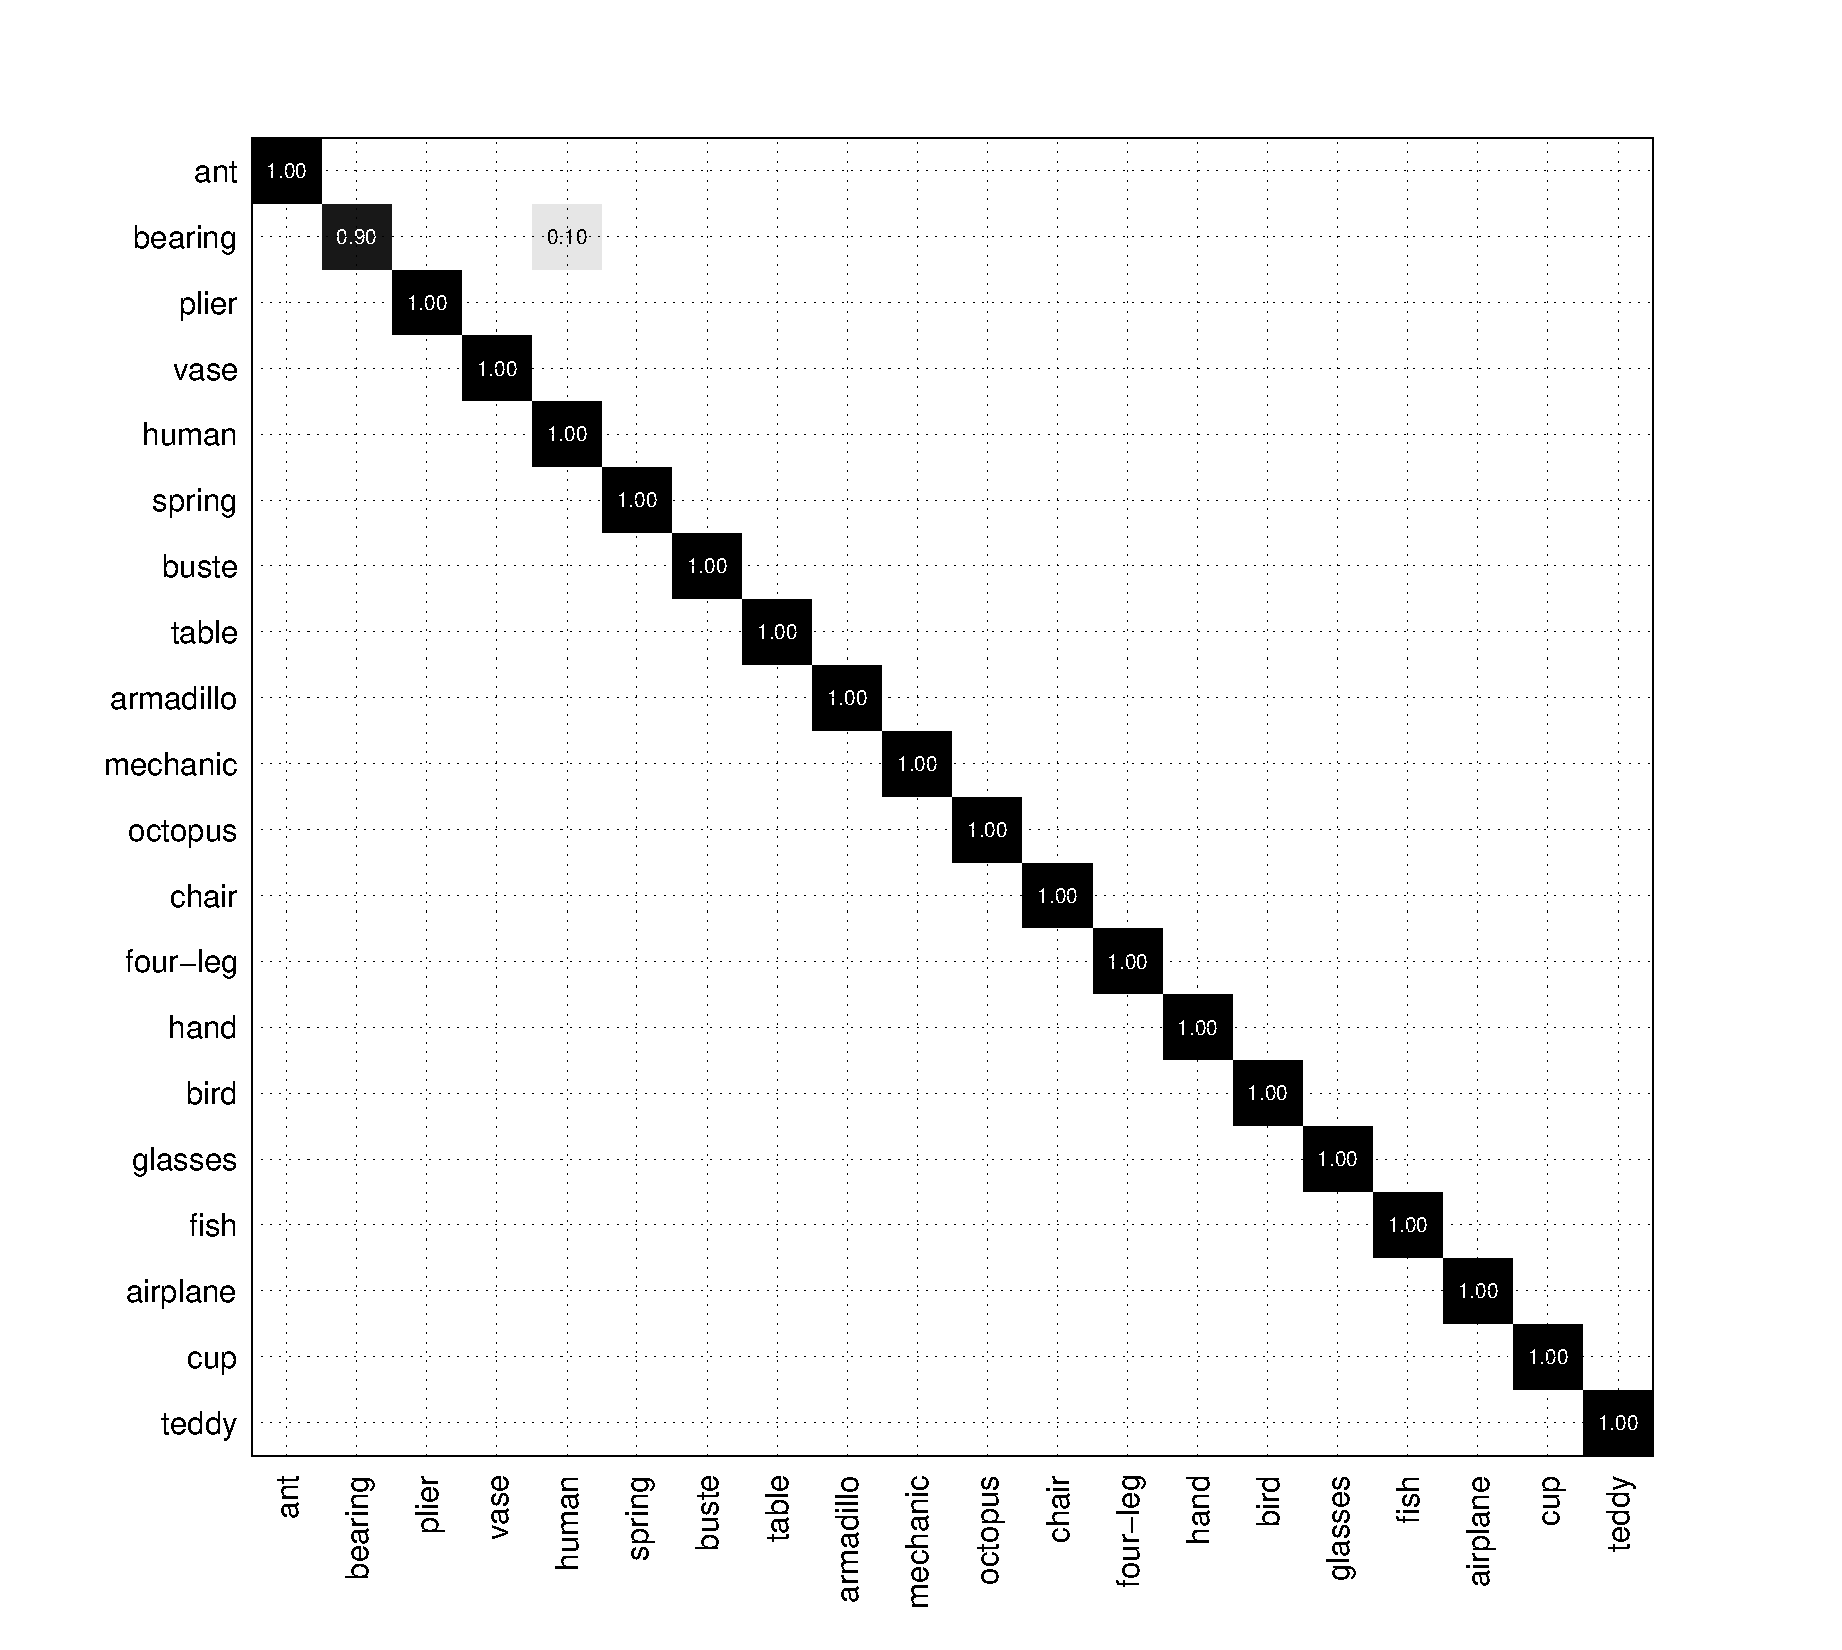
\includegraphics[width=0.98\linewidth]{figures/CM2007} 
\end{center} 
\vspace{-4mm}
\caption{在SHREC 2007上用提出的方法计算混淆矩阵。.} \label{fig_cm_shrec2007}
\end{figure*}

\begin{table}[hptb]
\caption{提出的方法的平均分类结果(\%)}\label{table_classification_results_3}
\centering
\begin{tabular}{lccc}  % {lccc} c
\hline \hline
特征                 &SHREC 2007     &SHREC 2011         & McGill \\ 
\hline
几何特征   &82.00          &70.00              & 81.69    \\ 
视觉特征       &89.22          &73.75              & 85.22\\  

3D MMF                  &\textbf{99.50} &\textbf{95.40}     &\textbf{97.47}\\  
\hline  \hline       
\end{tabular}

\end{table}

\begin{figure*}[hptb]
\begin{center}
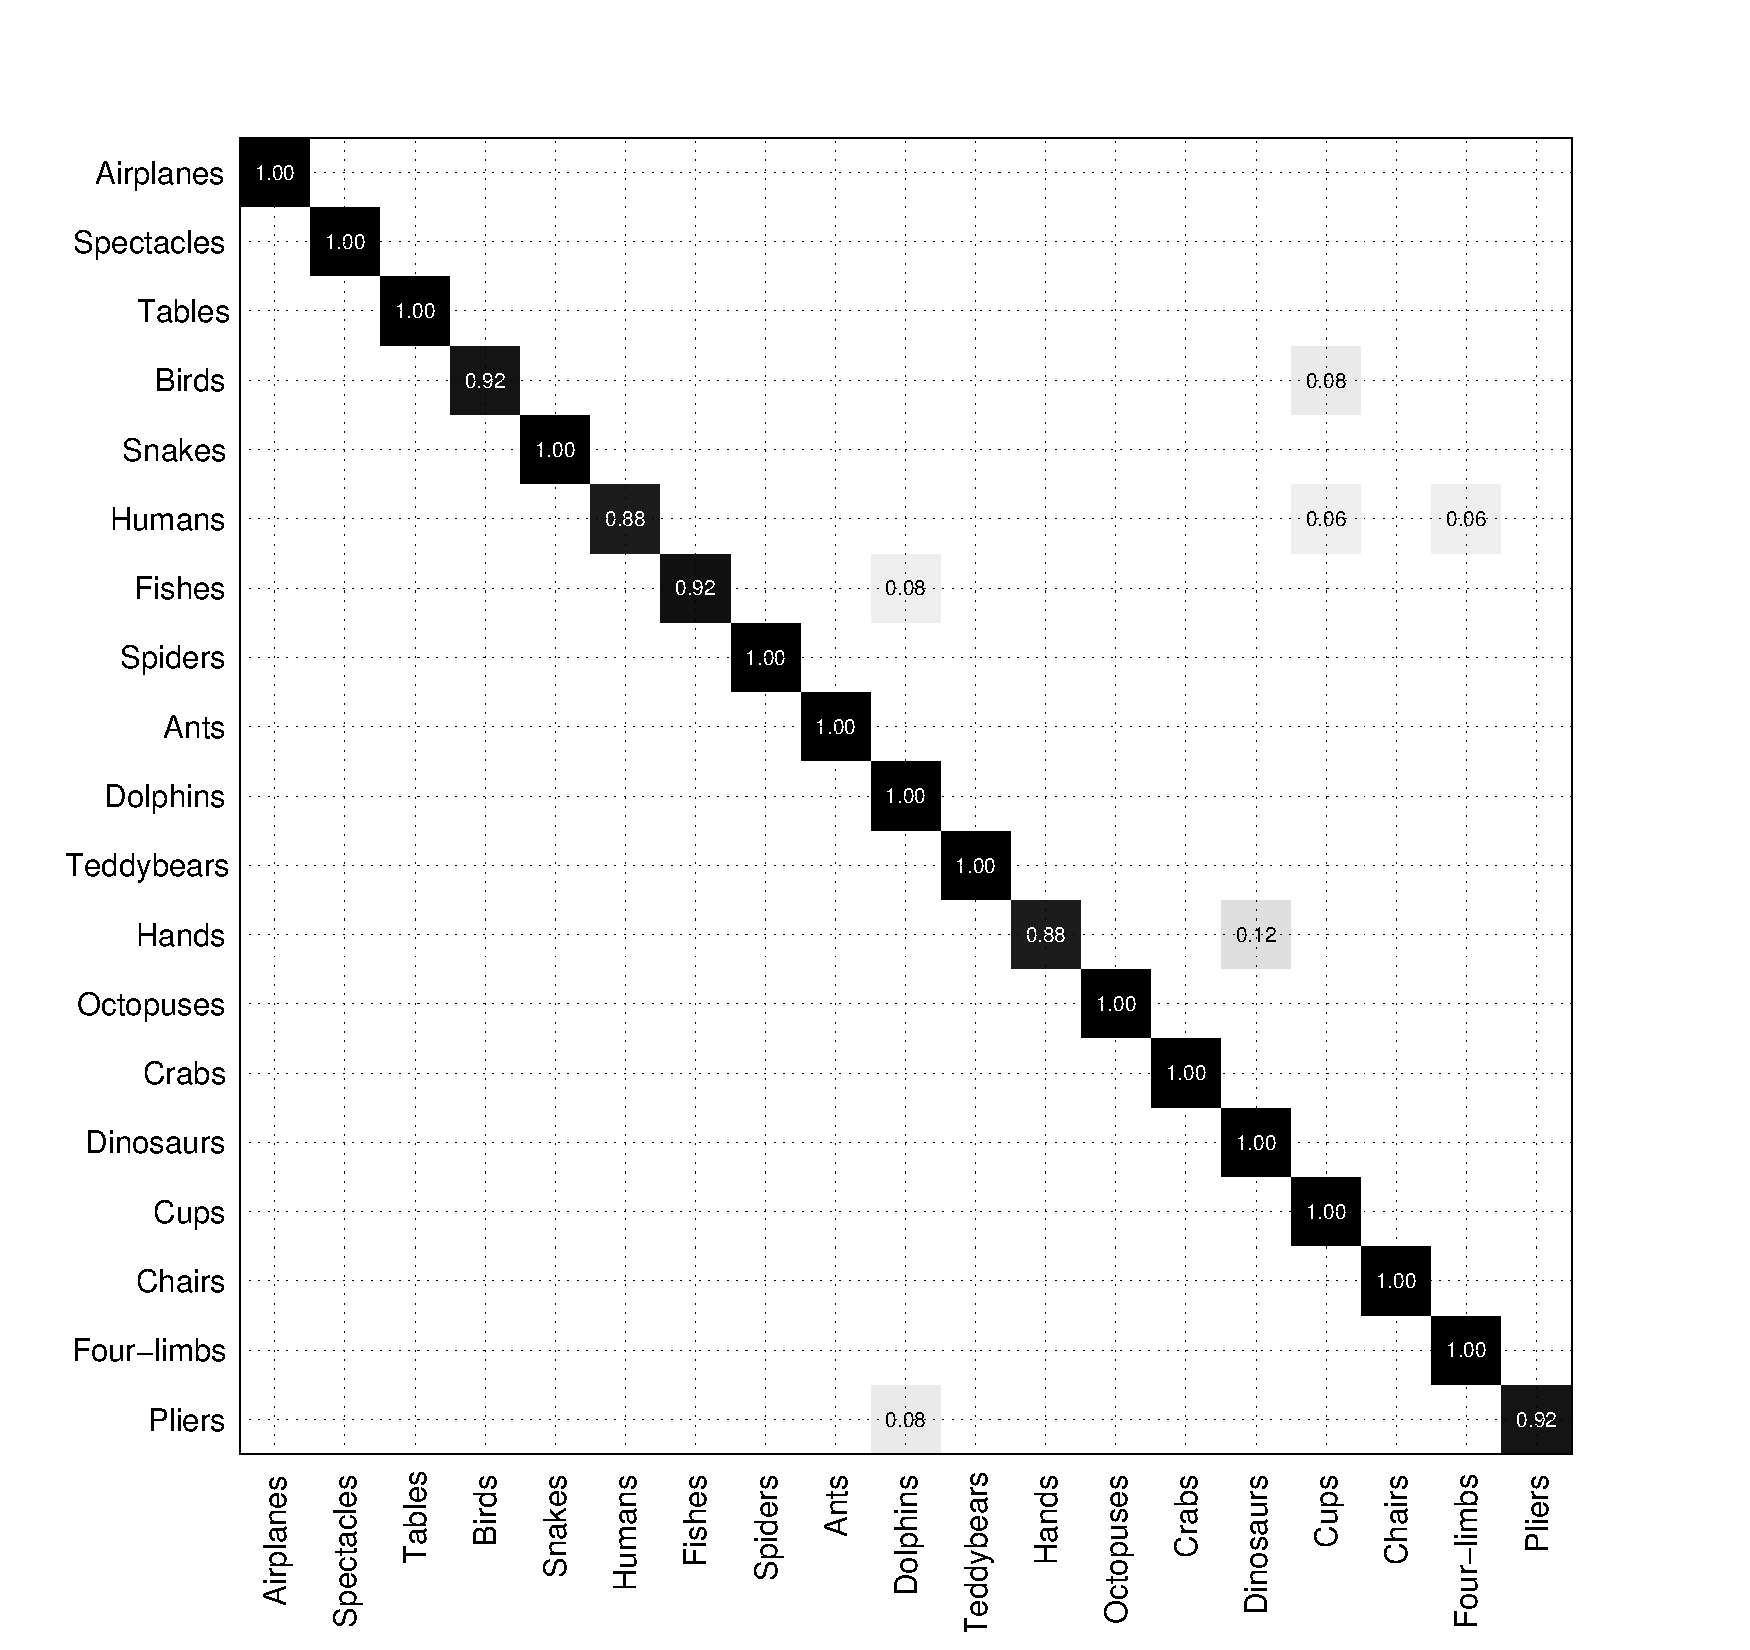
\includegraphics[width=0.98\linewidth]{figures/CMmcgill}
\end{center} 
\vspace{-4mm}
\caption{在McGill上用提出的方法计算混淆矩阵。} \label{fig_cm_mcgill}
\end{figure*}

我们分别在SHREC 2007,SHREC 2011和McGill数据集上进行分类实验,分别具有视觉描述符,几何描述符描述符和三维MMF三种类型的特征。 在表\ref {table_classification_results_3}中可以看到每个类型特征的平均分类精度。从表\ref {table_classification_results_3}中,我们可以清楚地得出结论,与仅使用单一模态特征所获得的结果相比,3D MMF实现了更好的分类性能。 这可以由几何和基于视图的模态只反映3D模型的部分属性这一事实来解释,因此,当考虑到两种不同的模态时,我们可以获得更多的判别力。 在三个数据集中,SHREC 2011的结果由于小的形状变化导致不敏感的描述,所以在SHREC 2011上的结果具有最低的准确性。 从表格中我们注意到几何描述符描述符的分类性能比视觉描述符差。 主要原因在于体素化操作像拓扑关系一样丢失了某些信息,导致性能不足,尽管体素化很容易用于CDBN模型的三维形状分析。
\begin{figure*}[hptb]
\begin{center}
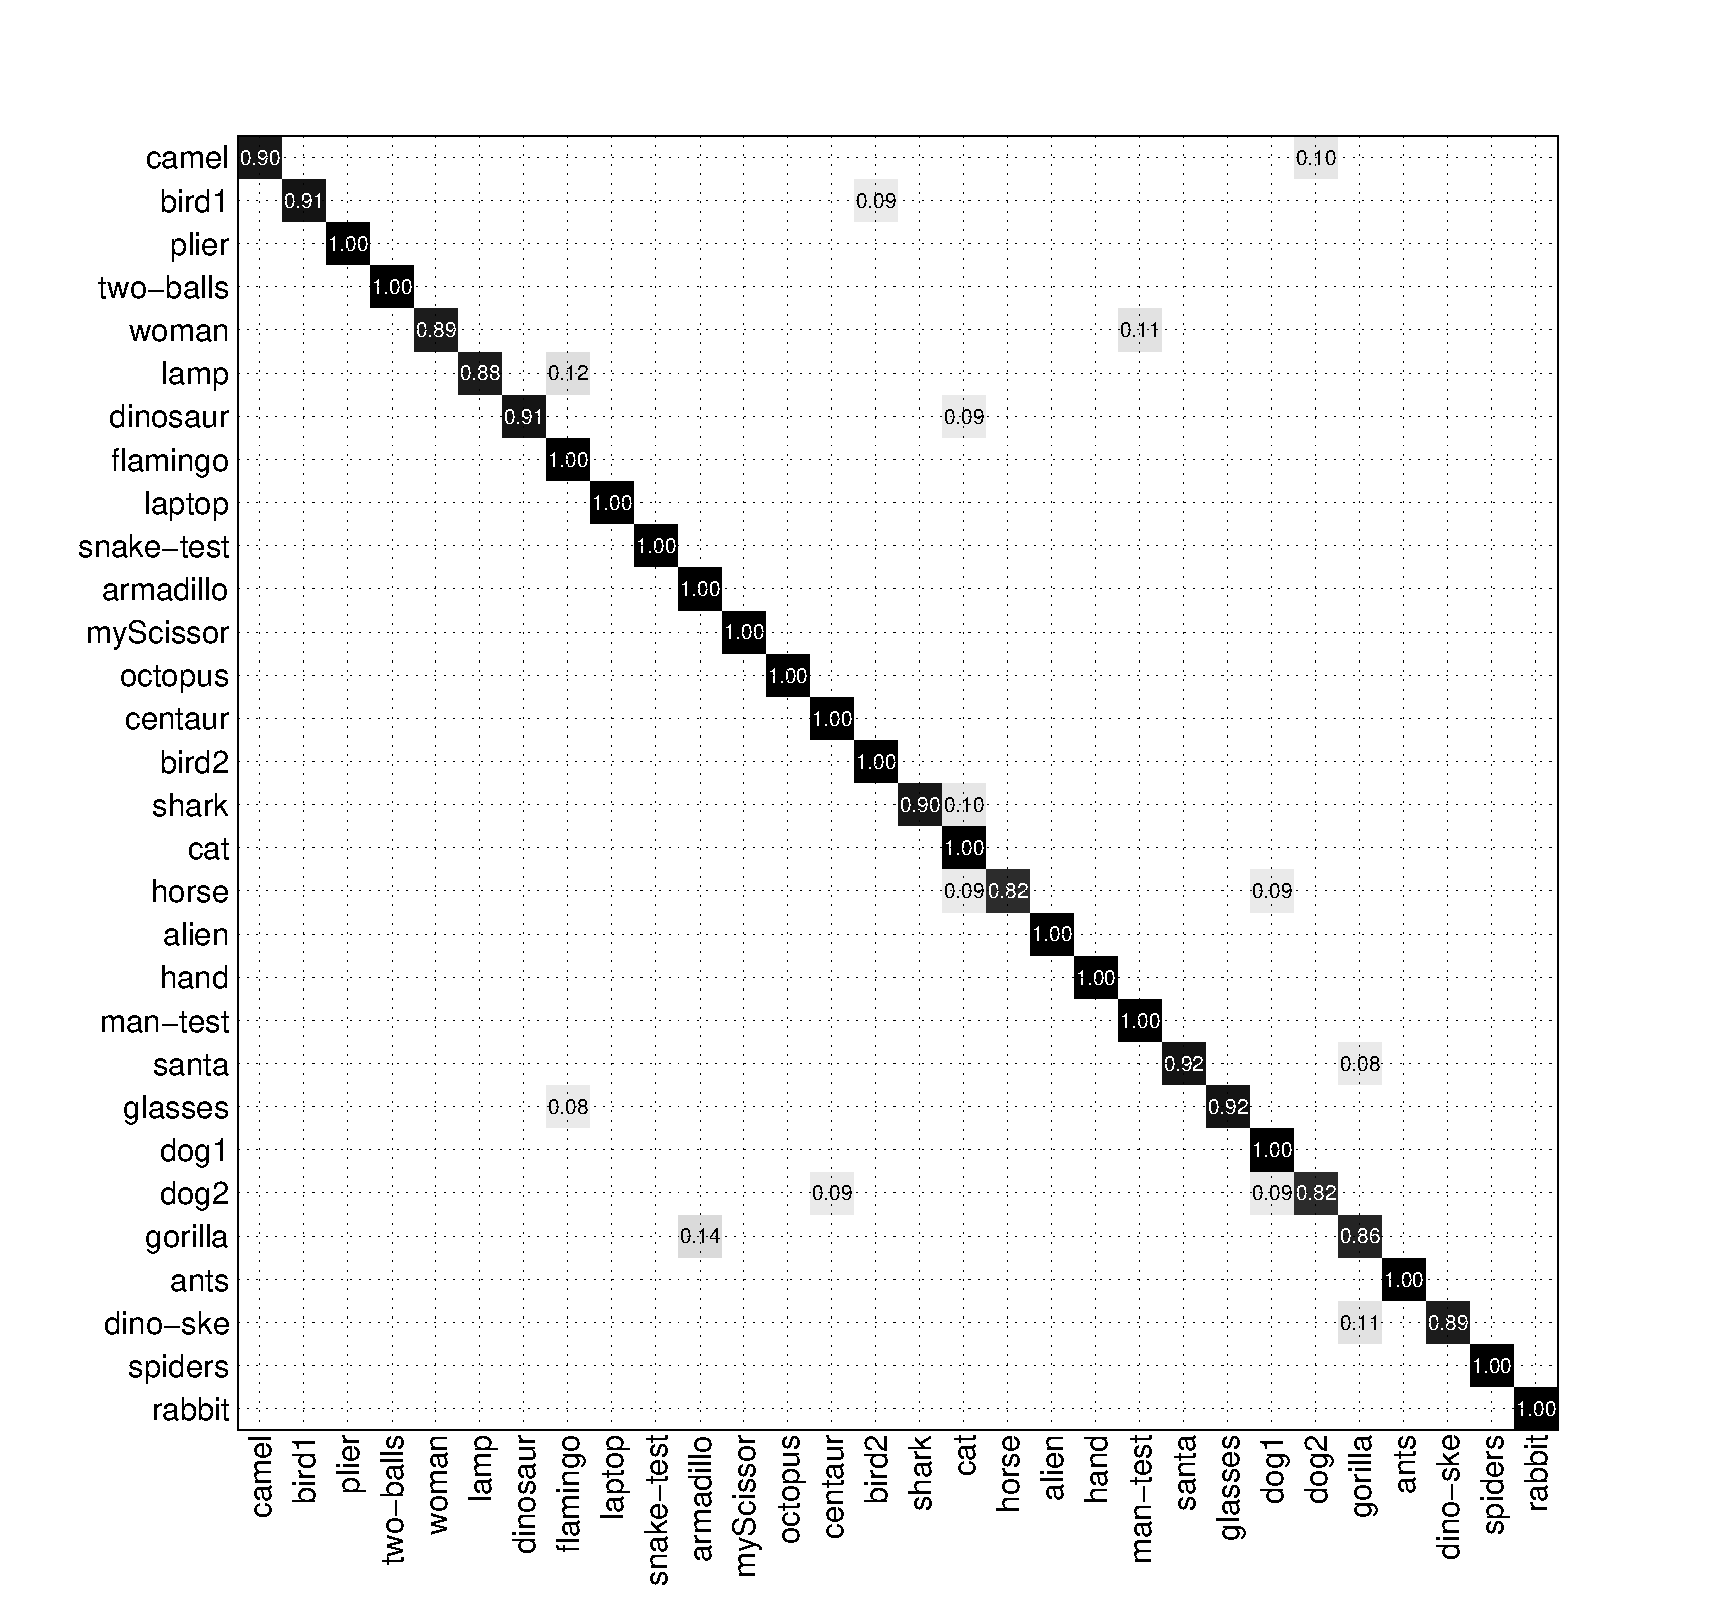
\includegraphics[width=0.98\linewidth]{figures/CM2011}
\end{center} 
\vspace{-4mm}
\caption{在SHREC 2011上用提出的方法计算混淆矩阵。} \label{fig_cm_shrec2011}
\end{figure*}


在机器学习领域,混淆矩阵是一种特定的表格布局,允许可视化算法的性能。 混淆矩阵包含有关分类系统完成的实际分类和预测分类的信息。 不同的颜色提供不同的概率。 为了进一步详细分析识别结果,在三维数据集上对三维数据集进行分类的混淆矩阵在图\ref {fig_cm_shrec2007}, \ref{fig_cm_mcgill}和\ref {fig_cm_shrec2011}可见。 从结果中可以得出结论,所提出的方法在SHREC2007、SHREC2011和McGill数据集的错误分类很低,之所以在SHREC2011上的表现相对于其他数据集稍微有点差,是因为SHREC2011数据集中包含许多十分相似的模型,不同的三维模型类间差距不大,因此实际上增加了分类的难度,但最终也取得了较好的结果,说明该方法具有广阔的应用前景。

\subsection{检索实验}

\begin{figure}[tbhp]
\begin{center}
\includegraphics[width=1\linewidth]{figures/PR2007}
\end{center} 
\vspace{-4mm}
\caption{一些最先进的方法和提出的方法在SHREC 2007的PR曲线.} \label{fig_rp_shrec2007}
\end{figure}

对于检索任务,有6个标准评估指标用于评估推荐方法的性能。 它们是 precision-recall curve, nearest neighbor (NN), first tier (FT), second tier (ST), E-measure (E), 和 discounted cumulative gain (DCG),详细的定义可以在\cite{shilane2004princeton}中找到。 我们使用在分类实验中训练的模型来计算每个3D形状的3D MMF。 等式 \eqref{cal_cal_distance}被用来描述两个模型之间的相似性。

%table
\begin{table}[tbhp]

\caption{SHREC 2007上的20,40,60和80个返回项目的精度值(\%)} \label{table_retrieval_shrec2007_precision}
\begin{center}
\begin{tabular}{cccccc}  % {lccc} 表示各列元素对齐方式,left-l,right-r,center-c
\hline  \hline
方法 			    &20     &40     &60     &80   \\ 
\hline
DLE \cite{giorgi2007watertight}   &54.6  &32.9  &24.1  &19.0   \\ 
MDD \cite{giorgi2007watertight}      &62.6  &36.6  &26.2  &20.5  \\
STT \cite{giorgi2007watertight}      &56.4  &34.6  &25.2  &19.9  \\
SI-MSC \cite{giorgi2007watertight}      &60.4  &36.6  &26.2  &20.5  \\
aMRG \cite{giorgi2007watertight}      &71.4  &41.4  &29.0  &22.5  \\
ERG \cite{barra20133d}      &62.4  &41.5  &30.5  &24.4  \\
3D MMF   &\textbf{97.2} &\textbf{49.4} &\textbf{33.0} &\textbf{24.8} \\  
\hline  \hline      % & 表示列的分隔线 
\end{tabular}
\end{center} 
\end{table}


\textbf{在SHREC 2007上的检索实验。} 我们在SHREC 2007数据集上进行检索实验来评估检索性能。我们的方法和一些最先进的方法的召回精度曲线如图\ref{fig_rp_shrec2007}所示,其中包括深度线编码(DLE)\cite{Giorgi2008SHape},多元密度描述符(MDD)\cite{Giorgi2008SHape},球面轨迹变换(STT)\cite{Giorgi2008SHape},轮廓交点和多尺度轮廓(SI-MSC)\cite{Giorgi2008SHape},增强的多分辨率Reeb图(aMRG)\cite{Giorgi2008SHape}和扩展的Reeb图(ERG)\cite{barra20133d}。数据集中所有模型的平均精度和召回率的数值分别列于表\ref {table_retrieval_shrec2007_precision}和\ref{table_retrieval_shrec2007_recall}中。我们列出了返回的20,40,60和80项的值,它们是每个类的大小的1,2,3和4倍。从图和表中可以清楚地看出,提出的方法达到最佳整体检索结果。检索实验采用来自体素的几何描述符和来自视图的视觉描述符。虽然只有视觉特征的表现明显优于竞争对手,但3D MMF仍然比它好。原因在于单一特征只能提供三维形状的特定方面信息,而所提出的方法则是基于形状和视图的形式信息融合。因此,3D MMF包含3D模型的内在属性和外在属性。同时3D MMF增加了类内相似度,降低了类间相似度。结果,检索性能得到改善。

%table
\begin{table}[tbhp]

\caption{SHREC 2007上的20,40,60和80个返回项目的召回率(\%)} \label{table_retrieval_shrec2007_recall}
\begin{center}
\begin{tabular}{cccccc}  % {lccc} 表示各列元素对齐方式,left-l,right-r,center-c
\hline  \hline
方法 			    &20     &40     &60     &80   \\ 
\hline
DLE \cite{giorgi2007watertight}   &54.6  &65.8  &72.4  &76.3   \\ 
MDD \cite{giorgi2007watertight}      &62.6  &73.2  &78.6  &82.1  \\
STT \cite{giorgi2007watertight}      &56.4  &69.2  &75.6  &79.8  \\
SI-MSC \cite{giorgi2007watertight}      &60.4  &73.2  &78.8  &82.2  \\
aMRG \cite{giorgi2007watertight}      &71.4  &82.8  &87.2  &90.2  \\
ERG \cite{barra20133d}      &62.4  &82.9  &91.6  &97.5  \\
3D MMF   &\textbf{97.2} &\textbf{98.8} &\textbf{99.1} &\textbf{99.3} \\  
\hline  \hline      % & 表示列的分隔线 
\end{tabular}
\end{center} 
\end{table}

%table
\begin{table}[tbhp]
\caption{在SHREC 2007上使用标准测量方法检测提出的方法的检索性能(\%)} \label{table_retrieval_shrec2007}
\begin{center}
\begin{tabular}{cccccc}  % {lccc} 表示各列元素对齐方式,left-l,right-r,center-c
\hline  \hline
特征 			    &NN     &FT     &ST     &E      &DCG \\ 
\hline
几何特征   &85.50  &57.82  &36.11  &50.70  &86.78 \\ 
视觉特征      &96.50  &86.98  &47.99  &68.61  &97.26 \\
3D MMF                  &\textbf{99.75} &\textbf{91.77} &\textbf{49.07} &\textbf{71.43} &\textbf{99.16}\\  
\hline  \hline      % & 表示列的分隔线 
\end{tabular}
\end{center} 
\end{table}


\begin{figure}[tbhp]
\begin{center}
\includegraphics[width=1.0\linewidth]{figures/PR2011}
\end{center} 
\vspace{-4mm}
\caption{一些最先进的方法和提出的方法在SHREC 2011的PR曲线} \label{fig_rp_shrec2011}
\end{figure}

\begin{figure}[tbhp]
\begin{center}
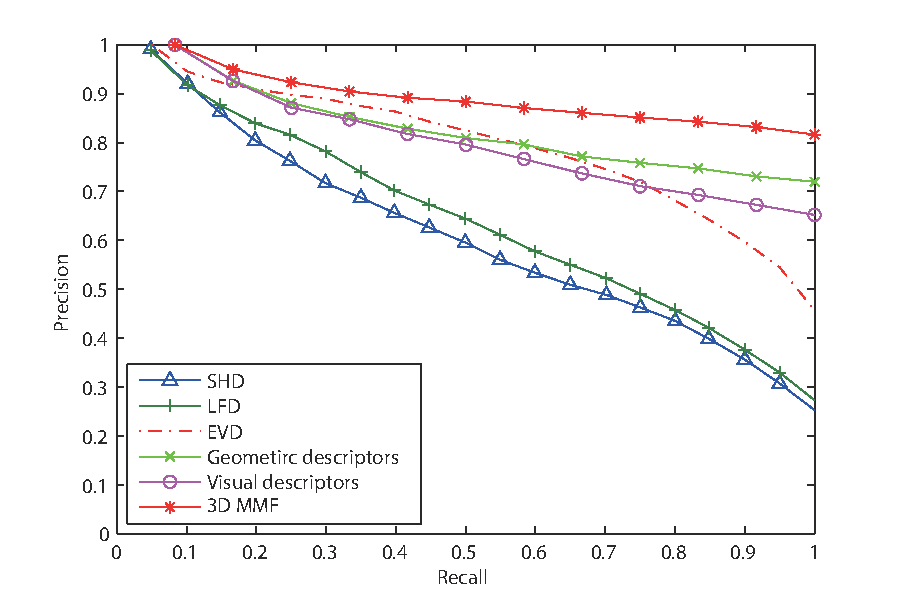
\includegraphics[width=1.0\linewidth]{figures/Mcgill_PR}
\end{center} 
\vspace{-4mm}
\caption{一些最先进的方法和提出的方法在McGill的PR曲线} \label{fig_rp_McGill}
\end{figure}

表\ref {table_retrieval_shrec2007}列出了数字评估结果。 从表格中我们可以清楚地看到,所有的措施都从使用单一模式特征到多模态特征得到了很大的改善。 NN,FT,ST,E,DCG指数的平均改善程度分别为8.75%,19.37%,7.02%,11.78%,7.14%,说明多模式融合法产生的三维MMF具有 提高检索性能的出色能力。




\textbf{SHREC 2011和McGill的检索实验。}
我们还对SHREC 2011和McGill数据集进行检索实验,以评估检索性能。 我们的方法和一些最先进的方法的召回精度曲线绘制在图\ref {fig_rp_shrec2011}和\ref {fig_rp_McGill}。 表\ref {table_retrieval_results_shrec2011}和\ref {table_retrieval_results_McGill}列出数字评估。 结果表明,该方法的检索性能具有广阔的应用前景。

%table
\begin{table}[tbhp]
\caption{在SHREC 2011上使用标准测量方法检测提出的方法的检索性能(\%)} \label{table_retrieval_results_shrec2011}
\begin{center}
\begin{tabular}{cccccc}  % {lccc} 表示各列元素对齐方式,left-l,right-r,center-c
\hline  \hline
特征                 &NN &FT &ST &E &DCG\\ 
\hline
几何特征  &85.50 &57.81 &36.11 &50.70 &86.78   \\ 
视觉特征     &96.83 &86.02 &46.51 &\textbf{89.39} &96.86\\                   
3D MMF              &\textbf{98.00} &\textbf{86.85} &\textbf{46.80} &67.76 &\textbf{97.35}\\  
\hline  \hline      % & 表示列的分隔线 
\end{tabular}
\end{center} 
\end{table}



%table
\begin{table}[tbhp]

\caption{在McGill上使用标准测量方法检测提出的方法的检索性能(\%)}\label{table_retrieval_results_McGill}
\begin{center}
\begin{tabular}{cccccc}  % {lccc} 表示各列元素对齐方式,left-l,right-r,center-c
\hline  \hline
特征                 &NN &FT &ST &E &DCG\\ 
\hline
几何特征   &88.84 &62.45 &37.68 &59.66 &88.37    \\ 
视觉特征      &87.30 &54.12 &36.23 &51.91 &86.51\\                   
3D MMF              &\textbf{92.12} &\textbf{73.19} &\textbf{42.12} &\textbf{68.55} &\textbf{92.38}\\  
\hline  \hline      % & 表示列的分隔线 
\end{tabular}
\end{center} 
\end{table}

\section{总结}
本节提出了一种新的三维形状识别与检索的多模态特征提取与融合方法。 首先,通过CDBN和CNN分别提取几何描述符和视觉描述符作为基于几何的特征和基于视图的特征。 然后采用两个DBN学习结构化的高层描述符。 此外,为了发现模式之间的深层相互关系,我们利用RBM来融合这些高级特征。 在分类和检索任务的标准基准上进行的实验已经证明,与最先进的方法相比,所提出的方法实现更好的性能。 实验结果表明,融合表示具有较强的判别能力,能够抑制类内变异,增强类间相似性分离。

与传统的计算机视觉形态分析方法不同,我们充分考虑了内在属性和外在视觉相似性。 另外,我们不是简单地融合几何和视觉特征来训练模型,相反,我们采取的策略是首先通过DBN学习高级特征,通过DBN去除特定于模态的信息,然后是高层特征融合学习形状分析的多模态特征。 通过使用这种策略,可以对基于几何的模型和基于视图的模态之间高度非线性的相关性进行全面建模。

\textbf{局限性。} 在生成几何描述符的过程中,网格尺寸越小,精度越高,但计算量呈指数增长。 因此,应该设计一个合适的方法来平衡这两个方面。在我们的框架下,为了学习三维形状的融合表示,我们将不同模式的高层特征连接起来。 然而,每个形态特征携带的信息并不完全相同,从SHREC 2007数据集上的实验可以看出,视觉描述符比几何描述符包含更多的信息。 因此,应寻求解决办法来表示不同形式的重要性。 此外,在所提出的方法中,深度学习的特征是全局性的,使得三维形状的局部信息或多或少地丢失。 因此,该方法难以应用于更复杂的任务,如分割,局部检索和对称检测。

\textbf {未来的工作。} 首先,目前我们只研究框架中的几何和视觉描述符。 为了更好地描述三维形状,我们将探索将各种形式的全局特征和局部特征相结合的可能性。 其次,研究其他方法可以保留更多的结构信息进行特征学习。第三,研究可以直接处理图形数据的深度学习方法,包括三维网格数据,communication network和traffic network,这将会引起其更广泛的应用和更好的性能。

